
\begin{frame}[ctb!]
\frametitle{Clay GDSM Sorption Sensitivity}
It is clear from Figures \ref{fig:KdSumFactor} and \ref{fig:KdSum} that 
for retardation coefficients greater than the threshold , the 
relationship between peak annual dose and retardation coefficient is a strong 
inverse one. 

\begin{figure}[ht]
\centering
\includegraphics[width=0.7\linewidth]{./nuclide_demonstration/Retardation_Summary_kd.eps}
\caption{$K_d$ sensitivity.  The peak annual dose due to an inventory, 
$N$, of each isotope.}
\label{fig:KdSum}
\end{figure}

\end{frame}
